% Provenance (never printed): see sources/outline_sources.md (Year 2: partial melting of the
% mantle; solidus and geotherm; decompression, hydration and heating; degree of melting;
% binary and ternary phase diagrams applied to rocks).
% Curves from figdata/bachelor-2/melting.py (Bowen 1915 diopside-anorthite, Bowen and
% Andersen 1914 forsterite-silica, Katz et al. 2003 melting of peridotite); exercise and
% problem values in the Book 4 scratch calculator calc/ch07.py.
\chapter{प्रावार का पिघलना}\label{ch:b2:mantle-melting}

प्रावार ठोस है। भूकंपीय अपरूपण तरंगें इसे ऊपर से नीचे तक पार करती हैं, और
इससे ऊपर लाया गया \omterm{def:b2:mantle-melting:peridotites}{पेरिडोटाइट} एक क्रिस्टलीय चट्टान है। फिर भी केवल महासागरीय कटकों के
अनुदिश ही यह हर वर्ष लगभग बीस घन किलोमीटर नई महासागरीय भूपर्पटी देता है,
जिसका हर घन मीटर किसी गलित से बना है। यह विरोधाभास तब घुल जाता है जब हम जान लेते हैं
कि प्रावार इसलिए नहीं पिघलता कि उसे गरम किया जाता है: वह इसलिए पिघलता है कि
उस पर दाब घटता है, या इसलिए कि उसमें जल मिलाया जाता है। कटक के नीचे
प्रावार उठता है, उसका दाब उसके तापमान से तेज़ी से घटता है, और वह अपना
गलन-वक्र पार कर लेता है; धँसते स्लैब के ऊपर, स्लैब से मुक्त जल उस
वक्र को प्रावार-कील के नीचे गिरा देता है। दोनों स्थितियों में चट्टान का केवल छोटा अंश
पिघलता है, और वह अंश, अपने अवशेष से अलग होकर, समुद्र-तल और
ज्वालामुखी चापों का बेसाल्ट बन जाता है। यह अध्याय पहले प्रावार की
चट्टान और उन प्रावस्था आरेखों का वर्णन करता है जो बताते हैं कि ऐसी चट्टानें कैसे पिघलती हैं, फिर
कटक के नीचे उठते प्रावार का अनुसरण उसकी बनाई भूपर्पटी की मोटाई तक करता है।
% ledger: white:crust (Book 3), data:pb2002 (Book 3), katz03:solidus

\begin{recall}
\textbf{रसायन-विज्ञान की पुस्तकों (द्वितीय वर्ष) से}: द्विघटकी प्रावस्था आरेख,
सॉलिडस और लिक्विडस, गलनक्रांतिक बिंदु, सर्वांगसम गलन, ठोस विलयन
और उत्तोलक नियम, जिसके अनुसार दो सहअस्तित्वी प्रावस्थाओं के अनुपात
समग्र संघटन से उनकी दूरियों के व्युत्क्रमानुपाती होते हैं।
\textbf{भौतिकी की पुस्तकों से}: विशिष्ट ऊष्मा, गुप्त ऊष्मा, एन्ट्रॉपी
और द्वितीय नियम, जिसके अनुसार उत्क्रमणीय रुद्धोष्म प्रक्रम एन्ट्रॉपी संरक्षित रखता है।
\textbf{पुस्तक 3 (स्नातक वर्ष 1) से}: मुख्य चट्टान-निर्माता खनिज, ओलिवीन,
पाइरॉक्सीन, गार्नेट और स्पिनेल, उनके ठोस विलयन और Mg संख्या;
प्रावार रुद्धोष्म, $\mathrm dT/\mathrm dz = \alpha gT/c_p$; महासागरीय भूपर्पटी,
हॉटस्पॉट से दूर \qty[uncertainty-mode=separate]{7.1 \pm 0.8}{km} मोटी और
किसी प्रावार-स्तंभ के क्रोड के ऊपर लगभग \qty{20}{km}; धँसते स्लैब और उनके द्वारा
ले जाया जाने वाला जल। \textbf{\cref{ch:b2:elements-in-the-earth} से}: \omterm{def:b2:elements-in-the-earth:morb-oib}{मध्य-महासागरीय कटक बेसाल्ट}
(MORB), विभाजन गुणांक और \omterm{def:b2:elements-in-the-earth:partition}{असंगत तत्त्व}।
\end{recall}

\section{प्रावार की चट्टान}\label{sec:b2:mantle-melting:rock}

प्रावार की चट्टान पृष्ठ तक दो रूपों में पहुँचती है: \omterm{def:b2:magma-emplacement:magma}{मैग्मा} द्वारा ऊपर लाए गए खंड,
ज़ेनोलिथ, और महाद्वीपों पर धकेली गई महासागरीय स्थलमंडल की परतों का आधार,
ओफ़ियोलाइट। इसका लगभग सारा भाग \omterm{def:b2:mantle-melting:peridotites}{पेरिडोटाइट} है।
% ledger: geo:peridotite (Book 2), tulane:ocean-basins (Book 2)

\begin{definition}[पेरिडोटाइट और उसके प्रकार]\label{def:b2:mantle-melting:peridotites}
\emph{पेरिडोटाइट}\index{पेरिडोटाइट} एक स्थूल-कणिक अल्ट्रामैफ़िक चट्टान है
जिसमें \qty{40}{\percent} से अधिक ओलिवीन होता है, शेष पाइरॉक्सीन और
थोड़ा-सा एक ऐलुमिनीयुक्त खनिज (स्पिनेल या गार्नेट)। \emph{ड्यूनाइट}\index{ड्यूनाइट}
में \qty{90}{\percent} से अधिक ओलिवीन होता है। इससे नीचे,
\emph{लर्ज़ोलाइट}\index{लर्ज़ोलाइट} में ऑर्थोपाइरॉक्सीन और क्लाइनोपाइरॉक्सीन दोनों होते हैं;
\emph{हार्ज़बर्गाइट}\index{हार्ज़बर्गाइट} में ऑर्थोपाइरॉक्सीन होता है पर
लगभग कोई क्लाइनोपाइरॉक्सीन नहीं; वेर्लाइट में क्लाइनोपाइरॉक्सीन होता है पर लगभग कोई
ऑर्थोपाइरॉक्सीन नहीं। \qty{40}{\percent} से कम ओलिवीन वाली चट्टानें पाइरॉक्सिनाइट हैं।
\end{definition}
% ledger: bgs:ultramafic

यह वर्गीकरण एक त्रिभुज पर पढ़ा जाता है जिसके कोने ओलिवीन,
ऑर्थोपाइरॉक्सीन और क्लाइनोपाइरॉक्सीन हैं (नीचे का चित्र): हर बिंदु एक चट्टान को दर्शाता है,
और तीनों भुजाओं से उसकी दूरियाँ तीनों खनिजों के अनुपात देती हैं।
कटकों के नीचे पिघलने वाले क्षीणित ऊपरी प्रावार के एक मॉडल संघटन में
\qty{57}{\percent} ओलिवीन,
\qty{28}{\percent} ऑर्थोपाइरॉक्सीन, \qty{13}{\percent} क्लाइनोपाइरॉक्सीन और
\qty{2}{\percent} स्पिनेल है: एक \omterm{def:b2:mantle-melting:peridotites}{लर्ज़ोलाइट}।
% ledger: liang21:dmm-mode

\begin{omfigure}
\centering
\begin{tikzpicture}[x=1.25cm, y=1.25cm, font=\scriptsize]
\coordinate (O) at (2.5,4.330); \coordinate (P) at (0,0); \coordinate (C) at (5,0);
\fill[green!8] (2.25,3.897) -- (2.75,3.897) -- (O) -- cycle;
\fill[orange!10] (1,1.732) -- (2.25,3.897) -- (2.75,3.897) -- (4,1.732) -- cycle;
\draw[thick] (O) -- (P) -- (C) -- cycle;
\draw (2.25,3.897) -- (2.75,3.897);
\draw (1,1.732) -- (4,1.732);
\draw (2.5,3.897) -- (1.25,1.732);
\draw (2.5,3.897) -- (3.75,1.732);
\node[anchor=south] at (O) {ओलिवीन};
\node[anchor=north east] at (P) {ऑर्थोपाइरॉक्सीन};
\node[anchor=north west] at (C) {क्लाइनोपाइरॉक्सीन};
\node[anchor=west] at (2.85,4.05) {ड्यूनाइट};
\draw (2.5,4.05) -- (2.8,4.05);
\node at (2.5,2.05) {लर्ज़ोलाइट};
\draw (1.85,3.0) -- (0.75,3.3) node[anchor=east] {हार्ज़बर्गाइट};
\draw (3.15,3.0) -- (4.25,3.3) node[anchor=west] {वेर्लाइट};
\node at (2.5,0.85) {पाइरॉक्सिनाइट};
\node[anchor=east] at (0.95,1.732) {\qty{40}{\percent} ओलिवीन};
\node[anchor=east] at (2.2,3.897) {\qty{90}{\percent}};
\fill[red!70!black] (2.12,2.52) circle (2pt);
\draw[red!70!black] (2.12,2.52) -- (4.4,2.52) node[anchor=west] {प्रावार मॉडल};
\end{tikzpicture}
\par\smallskip{\small \omterm{def:b2:mantle-melting:peridotites}{पेरिडोटाइटों} और पाइरॉक्सिनाइटों का उनके ओलिवीन, ऑर्थोपाइरॉक्सीन
और क्लाइनोपाइरॉक्सीन के अनुपातों के अनुसार वर्गीकरण (ब्रिटिश
भूवैज्ञानिक सर्वेक्षण की योजना के आधार पर)। दोनों ऊपरी भुजाओं के अनुदिश संकरी पट्टियों में
लगभग बिना क्लाइनोपाइरॉक्सीन (\omterm{def:b2:mantle-melting:peridotites}{हार्ज़बर्गाइट}) या बिना ऑर्थोपाइरॉक्सीन (वेर्लाइट) वाली चट्टानें हैं।
लाल बिंदु कटकों के नीचे का मॉडल ऊपरी प्रावार है (57, 28 और
\qty{13}{\percent}, उसके \qty{2}{\percent} स्पिनेल के बिना पुनः प्रसामान्यीकृत)।}
\end{omfigure}
% ledger: bgs:ultramafic, liang21:dmm-mode

तीनों \omterm{def:b2:mantle-melting:peridotites}{पेरिडोटाइट} तीन स्वतंत्र चट्टान-प्रकार नहीं हैं: वे एक ही प्रक्रम की
अवस्थाएँ हैं। जब \omterm{def:b2:mantle-melting:peridotites}{पेरिडोटाइट} पिघलता है, तो सबसे पहले क्लाइनोपाइरॉक्सीन और ऐलुमिनीयुक्त खनिज
खप जाते हैं (\cref{sec:b2:mantle-melting:decompression}), इसलिए गलित खो चुका \omterm{def:b2:mantle-melting:peridotites}{लर्ज़ोलाइट}
उनमें निर्धन हो जाता है; पर्याप्त पिघलने के बाद वह
\omterm{def:b2:mantle-melting:peridotites}{हार्ज़बर्गाइट} होता है, और लगभग सारा पाइरॉक्सीन खो चुकी चट्टान \omterm{def:b2:mantle-melting:peridotites}{ड्यूनाइट} है।
% ledger: katz03:melting

\begin{definition}[उर्वर और अवशिष्ट प्रावार]\label{def:b2:mantle-melting:fertility}
\emph{उर्वर प्रावार}\index{उर्वर प्रावार} वह \omterm{def:b2:mantle-melting:peridotites}{पेरिडोटाइट} है, प्रायः
\omterm{def:b2:mantle-melting:peridotites}{लर्ज़ोलाइट}, जिसमें अब भी वह क्लाइनोपाइरॉक्सीन और ऐलुमिनीयुक्त खनिज है जिनसे
बेसाल्ट बनता है। \emph{अवशिष्ट प्रावार}\index{अवशिष्ट प्रावार} वह
\omterm{def:b2:mantle-melting:peridotites}{पेरिडोटाइट} है जो उससे गलित निकाल लिए जाने के बाद पीछे बचता है:
क्लाइनोपाइरॉक्सीन, ऐलुमिनियम, कैल्सियम और \omterm{def:b2:elements-in-the-earth:partition}{असंगत तत्त्वों} में निर्धन,
ओलिवीन में समृद्ध और ऊँची Mg संख्या वाला।
\end{definition}

\cref{ch:b2:isotope-geochemistry} का समस्थानिक \omterm{def:b2:isotope-geochemistry:reservoirs}{क्षीणित प्रावार} एक भंडार है,
जो अपने अनुपातों से परिभाषित है; \omterm{def:b2:mantle-melting:fertility}{अवशिष्ट प्रावार} एक चट्टान है, जो इससे परिभाषित है कि उसने क्या खोया।
दोनों जुड़े हुए हैं, क्योंकि \omterm{def:b2:isotope-geochemistry:reservoirs}{क्षीणित प्रावार} इसीलिए क्षीणित है कि उससे बहुत पहले गलित
निकाला गया था, पर एक को द्रव्यमान स्पेक्ट्रोमीटर में पढ़ा जाता है और दूसरे को
सूक्ष्मदर्शी के नीचे।

\section{चट्टानों के प्रावस्था आरेख}\label{sec:b2:mantle-melting:diagrams}

चट्टान खनिजों का मिश्रण है, और वह किसी एक बिंदु पर नहीं, तापमानों के एक परास में
पिघलती है। इसका वर्णन करने वाले आरेख पहले शुद्ध संश्लिष्ट खनिजों के
मिश्रणों पर मापे गए थे: एक छोटे आवेश को ज्ञात तापमान पर तब तक रखा जाता जब तक वह
साम्य में न आ जाए, फिर उसे शमित करके सूक्ष्मदर्शी के नीचे काँच, जो
द्रव था, और क्रिस्टल खोजे जाते।

\subsection*{एक द्विघटकी गलनक्रांतिक: डायोप्साइड और एनॉर्थाइट}

बेसाल्ट मूलतः एक कैल्सियमी प्लैजियोक्लेज़ और एक क्लाइनोपाइरॉक्सीन से बना है, और
बोवेन ने इसके सबसे सरल मॉडल के रूप में शुद्ध एनॉर्थाइट और डायोप्साइड चुने। मिलाकर गरम करने पर
वे एक साधारण गलनक्रांतिक
तंत्र बनाते हैं (नीचे का चित्र): डायोप्साइड \qty{1391.5}{\celsius} पर पिघलता है और एनॉर्थाइट
\qty{1550}{\celsius} पर, पर द्रव्यमान से \qty{58}{\percent} डायोप्साइड और
\qty{42}{\percent} एनॉर्थाइट का मिश्रण \qty{1270}{\celsius} पर पूरी तरह पिघल जाता है।
% ledger: bowen15:di-an

\begin{omfigure}
\centering
\begin{tikzpicture}
\begin{axis}[omrecord, width=0.78\linewidth, height=6cm,
  xmin=0, xmax=100, ymin=1200, ymax=1600,
  xlabel={एनॉर्थाइट (द्रव्यमान से \unit{\percent})}, ylabel={तापमान (\unit{\celsius})},
  y tick label style={/pgf/number format/1000 sep={}},
  tick label style={font=\scriptsize}, label style={font=\small}]
\addplot[very thick, black] table[x=x_an, y=T] {figdata/out/bachelor-2-melting-di-an-liq.dat};
\addplot[only marks, mark=*, mark size=1.6pt, blue!70!black] table[x=x_an, y=T] {figdata/out/bachelor-2-melting-di-an-data.dat};
\draw[thick] (axis cs:0,1270) -- (axis cs:100,1270);
\draw[densely dotted, red!70!black, thick] (axis cs:20,1590) -- (axis cs:20,1270);
\draw[->, red!70!black, thick] (axis cs:20,1350) -- (axis cs:41,1272);
\fill[red!70!black] (axis cs:20,1350) circle (1.6pt);
\node[font=\scriptsize] at (axis cs:55,1500) {द्रव};
\node[font=\scriptsize, align=center] at (axis cs:10,1300) {डायोप्साइड\\+ द्रव};
\node[font=\scriptsize, align=center] at (axis cs:72,1360) {एनॉर्थाइट + द्रव};
\node[font=\scriptsize] at (axis cs:68,1235) {डायोप्साइड + एनॉर्थाइट};
\node[font=\scriptsize, anchor=north east] at (axis cs:41,1267) {E, \qty{1270}{\celsius}};
\node[font=\scriptsize, anchor=west, red!70!black] at (axis cs:21,1360) {पहला डायोप्साइड};
\end{axis}
\end{tikzpicture}
\par\smallskip{\small वायुमंडलीय दाब पर डायोप्साइड--एनॉर्थाइट तंत्र,
बोवेन (1915) के शमन-प्रयोगों से: लिक्विडस तापमान (बिंदु, शमन-अंतरालों के
मध्यबिंदु) और गलनक्रांतिक E। लाल रंग में, \qty{20}{\percent} एनॉर्थाइट वाले
द्रव का शीतलन: डायोप्साइड \qty{1350}{\celsius} से क्रिस्टलित होता है,
द्रव लिक्विडस के अनुदिश E तक नीचे जाता है, और शेष वहाँ दोनों खनिजों के
मिश्रण के रूप में क्रिस्टलित होता है।}
\end{omfigure}
% ledger: bowen15:di-an

ऊपर से पढ़ने पर आरेख क्रिस्टलन का क्रम बताता है। \qty{20}{\percent} एनॉर्थाइट वाला
द्रव \qty{1350}{\celsius} पर डायोप्साइड क्रिस्टलित करने लगता है; द्रव,
डायोप्साइड खोते हुए, एनॉर्थाइट में समृद्ध होता जाता है और लिक्विडस के अनुदिश
तब तक नीचे जाता है जब तक गलनक्रांतिक तक न पहुँच जाए, जहाँ एनॉर्थाइट डायोप्साइड से
जुड़ जाता है और तापमान \qty{1270}{\celsius} पर तब तक रहता है जब तक सारा द्रव
समाप्त न हो जाए। नीचे से पढ़ने पर यह बताता है कि चट्टान कैसे पिघलती है: दोनों खनिजों के
अनुपात कुछ भी हों, पहला द्रव \qty{1270}{\celsius} पर प्रकट होता है और उसका
संघटन गलनक्रांतिक होता है। प्रावार के लिए यह पहला पाठ है। किसी चट्टान के पहले गलित का
संघटन चट्टान का संघटन नहीं होता: उसका संघटन उन खनिजों से तय होता है जिनसे वह
पिघलता है, और वह उन सभी के गलनांकों से काफ़ी नीचे के तापमान पर
प्रकट होता है।

\subsection*{असर्वांगसम गलन: फ़ॉर्स्टेराइट और सिलिका}

कुछ खनिज अपने ही संघटन वाले द्रव में नहीं पिघलते।

\begin{definition}[असर्वांगसम गलन, पेरिटेक्टिक बिंदु]\label{def:b2:mantle-melting:peritectic}
कोई खनिज \emph{असर्वांगसम गलन}\index{असर्वांगसम गलन} दिखाता है जब
गरम करने पर वह अपने ही संघटन वाले द्रव में पिघलने के बजाय एक अन्य ठोस और भिन्न
संघटन वाले एक द्रव में टूट जाता है। द्विघटकी
प्रावस्था आरेख पर, वह बिंदु जहाँ यह द्रव दोनों ठोसों के साथ सहअस्तित्व में होता है,
\emph{पेरिटेक्टिक बिंदु}\index{पेरिटेक्टिक बिंदु} है: गलनक्रांतिक के विपरीत, यह
दोनों ठोसों के संघटनों के बीच नहीं पड़ता।
\end{definition}

एन्स्टेटाइट, मैग्नीशियमी ऑर्थोपाइरॉक्सीन \ce{MgSiO3}, असर्वांगसम रूप से पिघलता है।
वायुमंडलीय दाब पर यह \qty{1557}{\celsius} पर फ़ॉर्स्टेराइट,
\ce{Mg2SiO4}, और स्वयं से थोड़े अधिक सिलिका-समृद्ध एक द्रव में टूटता है; केवल
\qty{1577}{\celsius} पर सारा फ़ॉर्स्टेराइट घुल चुका होता है (नीचे का चित्र)। बोवेन
और एंडरसन ने 1914 में पाया कि यह विघटन \qty{5.5}{\percent}
फ़ॉर्स्टेराइट और \qty{94.5}{\percent} द्रव देता है, जैसा उत्तोलक नियम
तीनों संघटनों से पूर्वानुमानित करता है (\cref{exo:b2:mantle-melting:6})। सिलिका की ओर और आगे, एन्स्टेटाइट और
क्रिस्टोबलाइट एक गलनक्रांतिक पर, \qty{1543}{\celsius} पर, साथ पिघलते हैं।
% ledger: bowen14:mgo-sio2

\begin{omfigure}
\centering
\begin{tikzpicture}
\begin{axis}[omrecord, width=0.78\linewidth, height=6cm,
  xmin=40, xmax=66, ymin=1450, ymax=1950,
  xlabel={\ce{SiO2} (द्रव्यमान से \unit{\percent})}, ylabel={तापमान (\unit{\celsius})},
  y tick label style={/pgf/number format/1000 sep={}},
  tick label style={font=\scriptsize}, label style={font=\small}]
\addplot[very thick, black] table[x=x_sio2, y=T] {figdata/out/bachelor-2-melting-fo-sio2-liq.dat};
\addplot[very thick, black, dashed] table[x=x_sio2, y=T] {figdata/out/bachelor-2-melting-fo-sio2-fo.dat};
\draw[thick] (axis cs:42.71,1450) -- (axis cs:42.71,1890);
\draw[thick] (axis cs:42.71,1557) -- (axis cs:60.86,1557);
\draw[thick] (axis cs:59.85,1450) -- (axis cs:59.85,1557);
\draw[thick] (axis cs:59.85,1543) -- (axis cs:66,1543);
\fill (axis cs:60.86,1557) circle (1.6pt);
\fill (axis cs:64.87,1543) circle (1.6pt);
\fill (axis cs:42.71,1890) circle (1.6pt);
\node[font=\scriptsize, anchor=south west] at (axis cs:42.9,1890) {फ़ॉर्स्टेराइट पिघलता है, \qty{1890}{\celsius}};
\node[font=\scriptsize] at (axis cs:56,1800) {द्रव};
\node[font=\scriptsize] at (axis cs:48,1680) {फ़ॉर्स्टेराइट + द्रव};
\node[font=\scriptsize] at (axis cs:51,1500) {फ़ॉर्स्टेराइट + एन्स्टेटाइट};
\node[font=\scriptsize, align=center] at (axis cs:63,1495) {एन्स्टेटाइट +\\क्रिस्टोबलाइट};
\node[font=\scriptsize, anchor=south] at (axis cs:61.3,1560) {P};
\node[font=\scriptsize, anchor=south] at (axis cs:64.87,1546) {E};
\node[font=\scriptsize, anchor=north, rotate=90] at (axis cs:42.71,1650) {\ce{Mg2SiO4}};
\node[font=\scriptsize, anchor=south, rotate=90] at (axis cs:59.85,1510) {\ce{MgSiO3}};
\end{axis}
\end{tikzpicture}
\par\smallskip{\small वायुमंडलीय दाब पर \ce{MgO}--\ce{SiO2} तंत्र का एक भाग,
बोवेन और एंडरसन (1914) से। एन्स्टेटाइट (\ce{MgSiO3})
पेरिटेक्टिक P, \qty{1557}{\celsius}, पर असर्वांगसम रूप से फ़ॉर्स्टेराइट और
\qty{60.9}{\percent} \ce{SiO2} वाले द्रव में पिघलता है; E एन्स्टेटाइट--क्रिस्टोबलाइट
गलनक्रांतिक है, \qty{1543}{\celsius}। फ़ॉर्स्टेराइट का लिक्विडस केवल एन्स्टेटाइट के
निकट मापा गया है: डैश वाला भाग फ़ॉर्स्टेराइट के गलनांक तक सीधा खींचा गया है।}
\end{omfigure}
% ledger: bowen14:mgo-sio2

पेरिटेक्टिक प्रावार के लिए दूसरा पाठ है। जब \omterm{def:b2:mantle-melting:peridotites}{पेरिडोटाइट} पिघलता है, तो उसका
ऑर्थोपाइरॉक्सीन बस घुलता नहीं: वह अवशेष को ओलिवीन और गलित को सिलिका
देता है। इसलिए गलित पाइरॉक्सीनों से अधिक सिलिका-समृद्ध होता है, और
अवशेष चट्टान से अधिक ओलिवीन-समृद्ध: \omterm{def:b2:mantle-melting:peridotites}{लर्ज़ोलाइट} से \omterm{def:b2:mantle-melting:peridotites}{हार्ज़बर्गाइट}
और \omterm{def:b2:mantle-melting:peridotites}{ड्यूनाइट} तक का पथ।

\subsection*{तीन घटक: त्रिघटकी आरेख}

वास्तविक चट्टानों में दो से अधिक खनिज होते हैं। तीन होने पर संघटन को एक
त्रिभुज चाहिए, और तापमान तीसरी विमा बन जाता है।

\begin{definition}[त्रिघटकी प्रावस्था आरेख, कोटेक्टिक रेखा, त्रिघटकी गलनक्रांतिक]\label{def:b2:mantle-melting:ternary}
\emph{त्रिघटकी प्रावस्था आरेख}\index{त्रिघटकी प्रावस्था आरेख} किसी दिए गए दाब पर
तीन घटकों वाले तंत्र के साम्यों को दर्शाता है: त्रिभुज का हर बिंदु
एक संघटन को दर्शाता है, कोने शुद्ध घटकों को, और
लिक्विडस पृष्ठ तापमान की समोच्च रेखाओं के रूप में या उन खनिजों के क्षेत्रों के रूप में
खींचा जाता है जो पहले क्रिस्टलित होते हैं। \emph{कोटेक्टिक रेखा}\index{कोटेक्टिक रेखा}
वह रेखा है जिसके अनुदिश द्रव एक साथ दो खनिजों में संतृप्त होता है और
ठंडा होते हुए दोनों को क्रिस्टलित करता है। कोटेक्टिक रेखाएँ त्रिभुज की भुजाओं पर स्थित द्विघटकी
गलनक्रांतिकों से नीचे उतरती हैं और \emph{त्रिघटकी
गलनक्रांतिक}\index{त्रिघटकी गलनक्रांतिक} पर मिलती हैं, वह न्यूनतम तापमान जिस पर द्रव रहता है,
जहाँ तीनों खनिज साथ क्रिस्टलित होते हैं।
\end{definition}

\begin{method}[त्रिघटकी आरेख पर क्रिस्टलन-पथ पढ़ना]\label{met:b2:mantle-melting:ternary}
त्रिभुज में समग्र संघटन $X$ और वह क्षेत्र खोजिए जिसमें वह पड़ता है:
उस क्षेत्र का खनिज पहले क्रिस्टलित होता है। जब तक केवल वही खनिज क्रिस्टलित होता है,
द्रव उस खनिज के कोने से सीधे दूर एक सीधी रेखा में चलता है,
$X$ से होकर, क्योंकि शुद्ध घटक हटाने से केवल उसका अनुपात बदलता है;
उत्तोलक नियम से क्रिस्टलों का द्रव्यमान-अंश $X$ से द्रव तक की दूरी है,
कोने से द्रव तक की दूरी से भाग दिया हुआ। जब द्रव किसी
\omterm{def:b2:mantle-melting:ternary}{कोटेक्टिक रेखा} तक पहुँचता है, तो दूसरा खनिज जुड़ता है और द्रव कोटेक्टिक के अनुदिश
ढाल पर नीचे \omterm{def:b2:mantle-melting:ternary}{त्रिघटकी गलनक्रांतिक} तक जाता है, जहाँ अंतिम द्रव क्रिस्टलित होता है। जो घटक
किसी भी क्रिस्टल में प्रवेश नहीं करता, वह द्रव में रहता है, इसलिए उसकी सांद्रता
शेष द्रव का अंश देती है: $f_{\text{द्रव}} = c_X/c_{\text{द्रव}}$।
\end{method}

\begin{omfigure}
\centering
\begin{tikzpicture}[x=1cm, y=1cm, font=\scriptsize]
\coordinate (A) at (3,5.196); \coordinate (B) at (0,0); \coordinate (C) at (6,0);
\coordinate (eAB) at (1.2,2.078); \coordinate (eAC) at (4.65,2.338);
\coordinate (eBC) at (3.9,0); \coordinate (E) at (3.45,1.299);
\coordinate (X) at (3.0,3.118); \coordinate (L) at (3.0,1.455);
\fill[green!8] (A) -- (eAB) -- (E) -- (eAC) -- cycle;
\fill[orange!10] (B) -- (eAB) -- (E) -- (eBC) -- cycle;
\fill[blue!7] (C) -- (eAC) -- (E) -- (eBC) -- cycle;
\draw[thick] (A) -- (B) -- (C) -- cycle;
\draw[very thick, -{Stealth[length=4pt]}] (eAB) -- ($(eAB)!0.55!(E)$);
\draw[very thick] ($(eAB)!0.5!(E)$) -- (E);
\draw[very thick, -{Stealth[length=4pt]}] (eAC) -- ($(eAC)!0.55!(E)$);
\draw[very thick] ($(eAC)!0.5!(E)$) -- (E);
\draw[very thick, -{Stealth[length=4pt]}] (eBC) -- ($(eBC)!0.55!(E)$);
\draw[very thick] ($(eBC)!0.5!(E)$) -- (E);
\draw[red!70!black, thick, dashed] (A) -- (X);
\draw[red!70!black, very thick, -{Stealth[length=4pt]}] (X) -- (L);
\draw[red!70!black, very thick, -{Stealth[length=4pt]}] (L) -- ($(L)!0.85!(E)$);
\fill[red!70!black] (X) circle (2pt); \fill[red!70!black] (L) circle (1.6pt);
\fill (E) circle (2pt);
\node[anchor=south] at (A) {A}; \node[anchor=north east] at (B) {B};
\node[anchor=north west] at (C) {C};
\node[anchor=west, red!70!black] at (3.1,3.2) {$X$};
\node[anchor=north east, red!70!black] at (2.95,1.42) {$L_1$};
\node[anchor=north west] at (3.5,1.25) {E};
\node[anchor=east] at (eAB) {$e_{AB}$}; \node[anchor=west] at (eAC) {$e_{AC}$};
\node[anchor=north] at (eBC) {$e_{BC}$};
\node at (2.35,2.75) {A क्षेत्र}; \node at (1.55,0.7) {B क्षेत्र}; \node at (4.9,0.7) {C क्षेत्र};
\end{tikzpicture}
\par\smallskip{\small एक \omterm{def:b2:mantle-melting:ternary}{त्रिघटकी गलनक्रांतिक} तंत्र (व्यवस्था-चित्र)। हर क्षेत्र में
वे द्रव हैं जिनसे उसका खनिज पहले क्रिस्टलित होता है; कोटेक्टिक रेखाएँ (तीर
घटते तापमान की ओर) द्विघटकी गलनक्रांतिकों $e$ से \omterm{def:b2:mantle-melting:ternary}{त्रिघटकी
गलनक्रांतिक} E तक जाती हैं। A क्षेत्र में स्थित द्रव $X$ A क्रिस्टलित करता है, और A
कोने से दूर तब तक चलता है जब तक $L_1$ पर A--B कोटेक्टिक से न मिले; तब A और B
साथ-साथ E तक क्रिस्टलित होते हैं, जहाँ C उनसे जुड़ता है (\cref{exo:b2:mantle-melting:11})।}
\end{omfigure}

तीन चट्टान-निर्माता खनिजों के तंत्र इसी तरह पढ़े जाते हैं। वे नियम जो तय करते हैं कि कितनी प्रावस्थाएँ सहअस्तित्व में रह सकती हैं,
और वे मुक्त-ऊर्जा पृष्ठ जिनसे ऐसे आरेख परिकलित होते हैं, इस शृंखला की
पुस्तक 5 (स्नातक वर्ष 3) के विषय हैं।

\section{सॉलिडस, रुद्धोष्म और पिघलने के तीन तरीके}\label{sec:b2:mantle-melting:solidus}

प्रावार के \omterm{def:b2:mantle-melting:peridotites}{पेरिडोटाइट} का एक सॉलिडस होता है, वह तापमान जिस पर उसका पहला गलित प्रकट होता है,
और उससे बहुत ऊपर एक लिक्विडस। दोनों दाब के साथ बढ़ते हैं। प्राकृतिक
\omterm{def:b2:mantle-melting:peridotites}{पेरिडोटाइटों} पर हुए प्रयोग, जिन्हें काट्ज़, स्पीगलमैन और लैंगम्यूर ने 2003 में संकलित करके फ़िट किया,
शुष्क सॉलिडस के लिए देते हैं
\[
  T_{\mathrm{s}}(P) = 1085.7 + 132.9\,P - 5.1\,P^2
\]
(डिग्री सेल्सियस में, $P$ गीगापास्कल में): पृष्ठ पर \qty{1086}{\celsius},
\qty{2}{GPa} पर \qty{1331}{\celsius}। इन्हीं गहराइयों पर प्रावार इससे अधिक गरम या
ठंडा होता है, इस पर निर्भर करते हुए कि वह कहाँ है, और प्रावारों की तुलना के लिए
गहराई का प्रभाव हटा दिया जाता है।
% ledger: katz03:solidus

\begin{definition}[प्रावार विभव तापमान]\label{def:b2:mantle-melting:tp}
\emph{प्रावार विभव तापमान}\index{प्रावार विभव तापमान} $T_p$
वह तापमान है जो संवहनशील प्रावार के किसी खंड का होता यदि उसे
प्रावार रुद्धोष्म के अनुदिश पृष्ठ तक लाया जाता, बिना ऊष्मा का विनिमय किए और
बिना पिघले।
\end{definition}

रुद्धोष्म के अनुदिश $\mathrm dT/\mathrm dP = \alpha T/(\rho c_p)$, जो ऊपर याद किए गए
प्रवणता $\alpha gT/c_p$ का दाब वाला रूप है, क्योंकि $\mathrm dP = \rho
g\,\mathrm dz$। $\alpha = \qty{4e-5}{K^{-1}}$, $\rho = \qty{3300}{kg/m^3}$
और $c_p = \qty{1000}{J/(kg.K)}$ के साथ यह लगभग \qty{20}{K} प्रति गीगापास्कल है,
एक गीगापास्कल प्रावार के \qty{30.9}{km} के बराबर होने पर (\cref{exo:b2:mantle-melting:3})। पुस्तक 3 (स्नातक वर्ष 1) ने
खनिज भौतिकी से प्रावार को लगभग \qty{1350}{\celsius} का विभव तापमान दिया था;
कटकों के नीचे के प्रावार के शैलिकीय आकलन 1280 से
\qty{1400}{\celsius} तक हैं।
% ledger: katz03:thermo, katsura:adiabat (Book 3), herzberg:tp (Book 3)

\begin{proposition}[विसंपीडन गलन का आरंभ]\label{prop:b2:mantle-melting:onset}
विभव तापमान $T_p$ वाला प्रावार, रुद्धोष्म $T = T_p + GP$ ($G$
स्थिर) के अनुदिश उठता हुआ, उस दाब $P_0$ पर पिघलने लगता है जहाँ रुद्धोष्म
सॉलिडस $T_{\mathrm s}(P) = a_1 + a_2P + a_3P^2$ से मिलता है, अर्थात इसका छोटा मूल:
\[
  -a_3P^2 + (G - a_2)P + (T_p - a_1) = 0 .
\]
$\Delta T_p$ से अधिक गरम प्रावार अधिक गहराई पर पिघलने लगता है, $\Delta P_0 \approx
\Delta T_p/(T_{\mathrm s}'(P_0) - G)$ से।
\end{proposition}

\begin{proof}
गहराई पर रुद्धोष्म सॉलिडस से ठंडा होता है, क्योंकि सॉलिडस अधिक
तीव्रता से बढ़ता है ($T_{\mathrm
s}' \approx \qty{110}{K/GPa}$, जबकि $G \approx 20$)। दोनों वक्र वहाँ काटते हैं जहाँ
$T_p + GP = a_1 + a_2P + a_3P^2$, जो पुनर्व्यवस्थित होकर द्विघात बन जाता है।
$T_p + GP_0 = T_{\mathrm s}(P_0)$ का अवकलन $\mathrm dT_p = (T_{\mathrm s}'(P_0) -
G)\,\mathrm dP_0$ देता है।
\end{proof}

$T_p = \qty{1350}{\celsius}$ के लिए आरंभ \qty{2.66}{GPa} पर है, लगभग
\qty{82}{km} नीचे, \qty{1403}{\celsius} पर; विभव तापमान का हर \qty{10}{\celsius}
इसे लगभग \qty{0.12}{GPa}, या \qty{3.6}{km}, खिसकाता है। नीचे का चित्र
सॉलिडस और रुद्धोष्म दिखाता है।

\begin{omfigure}
\centering
\begin{tikzpicture}
\begin{axis}[omrecord, width=0.8\linewidth, height=7cm,
  xmin=850, xmax=2000, ymin=0, ymax=6, y dir=reverse,
  xlabel={तापमान (\unit{\celsius})}, ylabel={दाब (\unit{GPa})},
  x tick label style={/pgf/number format/1000 sep={}},
  axis y line*=left,
  legend style={font=\scriptsize, at={(0.5,-0.2)}, anchor=north, legend columns=3},
  tick label style={font=\scriptsize}, label style={font=\small}]
\addplot[very thick, black] table[x=Ts, y=P_GPa] {figdata/out/bachelor-2-melting-pt.dat};
\addlegendentry{शुष्क सॉलिडस}
\addplot[thick, black, densely dotted] table[x=Tl, y=P_GPa] {figdata/out/bachelor-2-melting-pt.dat};
\addlegendentry{लर्ज़ोलाइट लिक्विडस}
\addplot[thick, black, dashed] table[x=Tq, y=P_GPa] {figdata/out/bachelor-2-melting-pt.dat};
\addlegendentry{लिक्विडस}
\addplot[thick, blue!70!black, dashdotted] table[x=wetsat, y=P_GPa] {figdata/out/bachelor-2-melting-pt.dat};
\addlegendentry{जल-संतृप्त सॉलिडस}
\addplot[thick, red!70!black] table[x=ad1350, y=P_GPa] {figdata/out/bachelor-2-melting-pt.dat};
\addlegendentry{रुद्धोष्म, $T_p$ = 1300, 1350, \qty{1450}{\celsius}}
\addplot[thin, red!70!black] table[x=ad1300, y=P_GPa] {figdata/out/bachelor-2-melting-pt.dat};
\addplot[thin, red!70!black] table[x=ad1450, y=P_GPa] {figdata/out/bachelor-2-melting-pt.dat};
\addplot[only marks, mark=*, mark size=2pt, red!70!black] table[x=T0, y=P0] {figdata/out/bachelor-2-melting-onset.dat};
\end{axis}
\begin{axis}[width=0.8\linewidth, height=7cm, xmin=850, xmax=2000,
  ymin=0, ymax=185.34, y dir=reverse, axis y line*=right, axis x line=none,
  ylabel={गहराई (\unit{km})}, tick label style={font=\scriptsize}, label style={font=\small}]
\end{axis}
\end{tikzpicture}
\par\smallskip{\small शुष्क \omterm{def:b2:mantle-melting:peridotites}{पेरिडोटाइट} के गलन-वक्र और जल-संतृप्त
सॉलिडस, काट्ज़ और अन्य (2003) के प्राचलीकरण से, तीन विभव तापमानों के
ठोस रुद्धोष्मों के साथ; बिंदु गलन का आरंभ दर्शाते हैं,
\qty{1300}{\celsius} के लिए \qty{2.08}{GPa}, \qty{1350}{\celsius} के लिए \qty{2.66}{GPa}
और \qty{1450}{\celsius} के लिए \qty{4.00}{GPa}। सॉलिडस और \omterm{def:b2:mantle-melting:peridotites}{लर्ज़ोलाइट} लिक्विडस के
बीच चट्टान पिघलती है जबकि वह अपना
क्लाइनोपाइरॉक्सीन बनाए रखती है। \qty{3300}{kg/m^3} वाले प्रावार के लिए गहराई-पैमाना।}
\end{omfigure}
% ledger: katz03:solidus, katz03:water, katz03:thermo

आरेख किसी चट्टान को उसके सॉलिडस से ऊपर लाने के तीन तरीके दिखाता है।

\begin{definition}[आंशिक, विसंपीडन और फ़्लक्स गलन]\label{def:b2:mantle-melting:melting}
\emph{आंशिक गलन}\index{आंशिक गलन} किसी चट्टान के एक अंश का पिघलना है,
उसके सॉलिडस और लिक्विडस के बीच। \emph{विसंपीडन
गलन}\index{विसंपीडन गलन} उस चट्टान का आंशिक गलन है जो उठती है,
और इसलिए ठंडा होने से तेज़ी से दाब खोती है, जब तक अपना सॉलिडस पार न कर ले।
\emph{फ़्लक्स गलन}\index{फ़्लक्स गलन}\index{जलयोजित गलन|see{फ़्लक्स गलन}},
या जलयोजित गलन, किसी वाष्पशील के, मुख्यतः जल के, मिलने से हुआ आंशिक गलन है,
जो सॉलिडस को चट्टान के तापमान से नीचे गिरा देता है। तीसरा
तरीका, किसी चट्टान को स्थिर दाब पर उसके सॉलिडस से ऊपर गरम करना, ऊष्मा के किसी बाहरी
स्रोत की माँग करता है, जैसे कोई गरम \omterm{def:b2:magma-emplacement:magma}{मैग्मा}।
\end{definition}

प्रावार में, जो ऊष्मा धीरे चालित करता है, तापन सबसे कम दक्ष है;
भूपर्पटी में बेसाल्टी \omterm{def:b2:magma-emplacement:magma}{मैग्मा} की ऊष्मा अपने आसपास की चट्टानों को पिघला सकती है
(\cref{ch:b2:crustal-melting})। विसंपीडन कटकों और हॉटस्पॉट को पोषित करता है;
\omterm{def:b2:mantle-melting:melting}{फ़्लक्स गलन} ज्वालामुखी चापों को।

\section{कटक के नीचे विसंपीडन गलन}\label{sec:b2:mantle-melting:decompression}

जब उठता प्रावार अपना सॉलिडस पार कर लेता है, तो वह उठता रहता है, और प्रश्न
यह बन जाता है कि वह कितना गलित बनाता है।

\begin{definition}[गलन-अंश]\label{def:b2:mantle-melting:fraction}
किसी आंशिक रूप से पिघली चट्टान का \emph{गलन-अंश}\index{गलन-अंश} $F$
उसके द्वारा बनाए गए गलित का द्रव्यमान है, उसके आरंभिक द्रव्यमान से भाग दिया हुआ। सॉलिडस
($F = 0$) और लिक्विडस ($F = 1$) के बीच, गलन-पृष्ठ पर तापमान
$T(P, F)$ का एक फलन है।
\end{definition}

पिघलने में ऊष्मा लगती है: गुप्त ऊष्मा, गलित के प्रति किलोग्राम $T\Delta S$, जहाँ
$\Delta S$ गलन की एन्ट्रॉपी है। उठता खंड अपने परिवेश से कोई ऊष्मा का विनिमय नहीं करता,
इसलिए गुप्त ऊष्मा उसके अपने तापमान से आती है, और वह स्थिर एन्ट्रॉपी वाले
उस पथ के अनुदिश उठता है जो सॉलिडस और लिक्विडस के बीच पड़ता है।

\begin{proposition}[समएन्ट्रॉपिक गलन-उत्पादकता]\label{prop:b2:mantle-melting:productivity}
बिना ऊष्मा-विनिमय के उठते प्रावार के लिए, विशिष्ट ऊष्मा $c_p$, तापीय
प्रसारता $\alpha$, घनत्व $\rho$ और गलन की एन्ट्रॉपी $\Delta S$ के साथ,
\emph{गलन-उत्पादकता}\index{गलन-उत्पादकता}, अर्थात दाब की प्रति एकांक गिरावट पर बना
गलित, है
\[
  -\frac{\mathrm dF}{\mathrm dP} =
  \frac{\dfrac{c_p}{T}\Big(\dfrac{\partial T}{\partial P}\Big)_F - \dfrac{\alpha}{\rho}}
       {\Delta S + \dfrac{c_p}{T}\Big(\dfrac{\partial T}{\partial F}\Big)_P}\,,
\]
जहाँ $T$ केल्विन में है।
\end{proposition}

\begin{proof}
आंशिक रूप से पिघली चट्टान की विशिष्ट एन्ट्रॉपी $\mathrm ds = c_p\,
\mathrm dT/T - (\alpha/\rho)\,\mathrm dP + \Delta S\,\mathrm dF$ से बदलती है: पहले दो
पद एक ठोस के हैं (दूसरा एक मैक्सवेल संबंध है, जो
भौतिकी की पुस्तकों से याद किया गया), तीसरा उस द्रव्यमान $\mathrm dF$ द्वारा प्राप्त एन्ट्रॉपी है जो
पिघलता है। उत्क्रमणीय रुद्धोष्म आरोहण $\mathrm ds = 0$ रखता है। गलन-पृष्ठ पर
$\mathrm dT = (\partial T/\partial P)_F\,\mathrm dP + (\partial
T/\partial F)_P\,\mathrm dF$। प्रतिस्थापित करने पर,
\[
  \Big[\frac{c_p}{T}\Big(\frac{\partial T}{\partial P}\Big)_F - \frac{\alpha}{\rho}\Big]\mathrm dP
  + \Big[\Delta S + \frac{c_p}{T}\Big(\frac{\partial T}{\partial F}\Big)_P\Big]\mathrm dF = 0,
\]
जो परिणाम है।
\end{proof}

अंश गलन-वक्रों की ढाल का रुद्धोष्म की ढाल पर आधिक्य है, यानी
चालक बल; हर में गुप्त ऊष्मा और वह ऊष्मा है जो पिघलती चट्टान का
तापमान गलन-अंतराल के अनुदिश बढ़ाने के लिए चाहिए, यानी ब्रेक। काट्ज़ और अन्य के
प्राचलों के साथ, $\Delta S = \qty{300}{J/(kg.K)}$, और ऐसे \omterm{def:b2:mantle-melting:fraction}{गलन-अंश} के साथ
जो सॉलिडस और \omterm{def:b2:mantle-melting:peridotites}{लर्ज़ोलाइट} लिक्विडस के बीच रैखिक रूप से बढ़ता है,
\qty{2}{GPa} पर उत्पादकता लगभग \qty{11}{\percent} प्रति गीगापास्कल है
(\cref{exo:b2:mantle-melting:8}): आरोहण का हर किलोमीटर चट्टान का लगभग एक-तिहाई प्रतिशत
पिघलाता है। उनका फ़िट किया हुआ गलन-फलन, जो गलित के पहले प्रतिशत को
धीरे-धीरे आने देता है, औसतन थोड़ा कम देता है, $T_p = \qty{1350}{\celsius}$ के लिए
आरंभ से पृष्ठ तक लगभग \qty{9}{\percent} प्रति गीगापास्कल। जब
क्लाइनोपाइरॉक्सीन खप जाता है, तो उत्पादकता गिरती है, उनके मॉडल में
$M_{\mathrm{cpx}}/(0.50 + 0.08P)$ के \omterm{def:b2:mantle-melting:fraction}{गलन-अंशों} के बाद, जो 13 से \qty{15}{\percent}
क्लाइनोपाइरॉक्सीन वाले प्रावार के लिए लगभग 25 से \qty{30}{\percent} हैं: \omterm{def:b2:mantle-melting:peridotites}{हार्ज़बर्गाइट} अवशेष
अनिच्छा से पिघलता है।
% ledger: katz03:melting, katz03:thermo

\begin{omfigure}
\centering
\begin{tikzpicture}
\begin{axis}[omrecord, width=0.62\linewidth, height=6.4cm,
  xmin=0, xmax=0.36, ymin=0, ymax=130, y dir=reverse,
  xlabel={गलन-अंश $F$}, ylabel={गहराई (\unit{km})},
  xtick={0,0.1,0.2,0.3},
  legend style={font=\scriptsize, at={(0.98,0.02)}, anchor=south east},
  tick label style={font=\scriptsize}, label style={font=\small}]
\addplot[thick, blue!70!black] table[x=F1300, y=z_km] {figdata/out/bachelor-2-melting-column.dat};
\addlegendentry{$T_p = \qty{1300}{\celsius}$}
\addplot[very thick, black] table[x=F1350, y=z_km] {figdata/out/bachelor-2-melting-column.dat};
\addlegendentry{$T_p = \qty{1350}{\celsius}$}
\addplot[thick, red!70!black, dashed] table[x=F1450, y=z_km] {figdata/out/bachelor-2-melting-column.dat};
\addlegendentry{$T_p = \qty{1450}{\celsius}$}
\end{axis}
\end{tikzpicture}
\par\smallskip{\small बिना ऊष्मा-विनिमय के उठते शुष्क \omterm{def:b2:mantle-melting:peridotites}{पेरिडोटाइट} के स्तंभ का \omterm{def:b2:mantle-melting:fraction}{गलन-अंश},
गलन के आरंभ से पृष्ठ तक, काट्ज़ और अन्य (2003) के गलन-फलन के साथ
एन्ट्रॉपी संरक्षित रखकर परिकलित,
\qty{15}{\percent} क्लाइनोपाइरॉक्सीन वाली चट्टान के लिए। \qty{1450}{\celsius} पर क्लाइनोपाइरॉक्सीन
\qty{25}{km} के निकट खप जाता है और वक्र अधिक खड़ा हो जाता है।}
\end{omfigure}
% ledger: katz03:melting, katz03:thermo

गलित वहीं नहीं रहता जहाँ वह बनता है। लगभग \qty{2900}{kg/m^3} पर वह
ठोस \omterm{def:b2:mantle-melting:peridotites}{पेरिडोटाइट}, \qty{3300}{kg/m^3}, से हल्का है, इसलिए वह अपने
अवशेष से अलग होकर उसमें से ऊपर उठता है; कटक के नीचे वह अक्ष की ओर एकत्र होता है।
भूपर्पटी प्रावार के पूरे एक क्षेत्र के गलितों से बनती है।
% ledger: katz03:thermo

\begin{proposition}[त्रिभुजाकार गलन-क्षेत्र की भूपर्पटी]\label{prop:b2:mantle-melting:triangle}
अर्ध-दर $U$ से फैलते कटक के नीचे, मान लीजिए प्रावार
चाल $U$ से ऊर्ध्वाधर उठता है, ऊँचाई $H$ वाले एक त्रिभुजाकार गलन-क्षेत्र से होकर, जिसका शीर्ष ऊपर
अक्ष के नीचे है और भुजाएँ \ang{45} पर हैं, और उसकी भुजाओं के आर-पार क्षैतिज रूप से चाल $U$ से
उसे छोड़ता है; मान लीजिए \omterm{def:b2:mantle-melting:fraction}{गलन-अंश} आधार पर $0$ से शीर्ष पर
$F_{\max}$ तक रैखिक रूप से बढ़ता है, सारा गलित भूपर्पटी में निकाला जाता है, और प्रावार तथा
भूपर्पटी का घनत्व समान है। तब भूपर्पटी
\[
  h_c = \int_0^H F(z)\,\mathrm dz = \tfrac12 F_{\max}H
\]
मोटी है, और एकत्रित गलित का माध्य \omterm{def:b2:mantle-melting:fraction}{गलन-अंश} $F_{\max}/2$ है।
\end{proposition}

\begin{proof}
$x$ अक्ष से और ऊँचाई $y$ आधार के ऊपर मापिए। प्रावार आधार में
$|x| \le H$ पर प्रवेश करता है और तब तक उठता है जब तक किसी भुजा से न मिले, $y = H - |x|$ पर, तब तक
$F = F_{\max}(H - |x|)/H$ तक पिघल चुका होता है। कटक की प्रति एकांक लंबाई और प्रति एकांक समय, बना गलित
$\int_{-H}^{H} U F\,\mathrm dx = 2UF_{\max}\int_0^H (1 - x/H)\,\mathrm dx =
UF_{\max}H$ है। भूपर्पटी दोनों ओर चाल $U$ से निकलती है: $2Uh_c = UF_{\max}H$।
संसाधित प्रावार $2UH$ है, इसलिए माध्य \omterm{def:b2:mantle-melting:fraction}{गलन-अंश} $UF_{\max}H/(2UH) =
F_{\max}/2$ है। अंत में $\int_0^H F_{\max}\,y/H\,\mathrm dy = F_{\max}H/2$।
\end{proof}

परिणाम प्रसार-दर पर निर्भर नहीं करता, जैसा प्रेक्षित है (पुस्तक 3,
स्नातक वर्ष 1)। $T_p = \qty{1350}{\celsius}$ के लिए ऊपर के चित्र का स्तंभ, अपनी
धीमी शुरुआत के साथ, $\int F\,\mathrm dz = \qty{9.0}{km}$ भूपर्पटी देता है, मापे गए
\qty{7.1}{km} से थोड़ी अधिक; \qty{50}{\celsius} ठंडा प्रावार
\qty{5.5}{km} देता है, और \qty{100}{\celsius} अधिक गरम \qty{19}{km}, जो किसी प्रावार-स्तंभ के
क्रोड के ऊपर के \qty{20}{km} के निकट है (नीचे का चित्र)। भूपर्पटी की मोटाई एक
तापमापी है, और संवेदनशील: चूँकि उत्पादकता स्थिर होने पर $h_c \propto P_0^2$,
दस डिग्री इसे लगभग दसवें भाग से बदल देते हैं (सप्ताहांत समस्या)।
% ledger: white:crust (Book 3)

\begin{omfigure}
\centering
\begin{tikzpicture}[x=1cm, y=1cm, font=\scriptsize]
\fill[blue!8] (-5.5,0.6) rectangle (5.5,0);
\fill[brown!35] (-5.5,0) -- (5.5,0) -- (5.5,-0.35) -- (-5.5,-0.35) -- cycle;
\fill[orange!25] (0,-0.45) -- (-3.6,-4.05) -- (3.6,-4.05) -- cycle;
\draw[densely dashed, thick] (-5.5,-4.05) -- (5.5,-4.05);
\node[anchor=north east] at (5.5,-4.55) {सॉलिडस पार: गलन आरंभ, गहराई $z_0$};
\foreach \s in {1,-1} {
  \draw[->, thick] (\s*0.4,0.35) -- (\s*1.6,0.35);
  \draw[gray, -{Stealth[length=3pt]}] (\s*1.8,-4.5) -- (\s*1.8,-2.45) .. controls (\s*1.8,-2.1) and (\s*2.1,-1.95) .. (\s*2.8,-1.95) -- (\s*5.3,-1.95);
  \draw[gray, -{Stealth[length=3pt]}] (\s*3.1,-4.5) -- (\s*3.1,-3.75) .. controls (\s*3.1,-3.4) and (\s*3.4,-3.25) .. (\s*4.1,-3.25) -- (\s*5.3,-3.25);
}
\draw[red!70!black, -{Stealth[length=3pt]}, thick] (-1.2,-3.0) -- (-0.3,-1.0);
\draw[red!70!black, -{Stealth[length=3pt]}, thick] (1.2,-3.0) -- (0.3,-1.0);
\draw[red!70!black, -{Stealth[length=3pt]}, thick] (0,-2.3) -- (0,-0.9);
\node[anchor=south] at (0,0.6) {कटक-अक्ष};
\node[anchor=west] at (1.7,0.35) {प्लेट, चाल $U$};
\node[anchor=west] at (-5.4,-0.2) {भूपर्पटी, $h_c$};
\node[align=center, inner sep=1pt] at (0,-3.3) {गलन-क्षेत्र};
\node[anchor=west, align=left] at (3.2,-2.55) {प्रावार की\\प्रवाह-रेखाएँ};
\node[anchor=east, align=right, red!70!black] at (-2.0,-2.6) {गलित अक्ष की\\ओर बहता है};
\end{tikzpicture}
\par\smallskip{\small कटक के नीचे एक त्रिभुजाकार गलन-क्षेत्र (व्यवस्था-चित्र, पैमाने के
अनुसार नहीं; वास्तव में $z_0$ भूपर्पटी की मोटाई का दस गुना है)। अक्ष के नीचे उठता
प्रावार $z_0$ पर अपना सॉलिडस पार करता है, उठते हुए पिघलता है, और पिघलना तब रोक देता है
जब चलती प्लेटों के नीचे उसका प्रवाह क्षैतिज हो जाता है; गलित ऊपर और
अक्ष की ओर रिसता है और भूपर्पटी बनाता है।}
\end{omfigure}

\begin{omfigure}
\centering
\begin{tikzpicture}
\begin{axis}[omrecord, width=0.72\linewidth, height=5.6cm,
  xmin=1250, xmax=1550, ymin=0, ymax=32,
  xlabel={प्रावार विभव तापमान $T_p$ (\unit{\celsius})},
  ylabel={बनी भूपर्पटी (\unit{km})},
  x tick label style={/pgf/number format/1000 sep={}},
  tick label style={font=\scriptsize}, label style={font=\small}]
\fill[blue!12] (axis cs:1250,6.3) rectangle (axis cs:1550,7.9);
\fill[red!12] (axis cs:1250,19) rectangle (axis cs:1550,21);
\addplot[very thick, black] table[x=Tp, y=h_km] {figdata/out/bachelor-2-melting-crust.dat};
\node[font=\scriptsize, anchor=west, blue!60!black] at (axis cs:1400,7.1) {सामान्य कटक, $7.1 \pm 0.8$};
\node[font=\scriptsize, anchor=east, red!60!black] at (axis cs:1440,20) {प्रावार-स्तंभ के ऊपर, $20 \pm 1$};
\end{axis}
\end{tikzpicture}
\par\smallskip{\small त्रिभुजाकार गलन-क्षेत्र द्वारा बनी भूपर्पटी की मोटाई,
अक्ष के अनुदिश $\int F\,\mathrm dz$, प्रावार के विभव तापमान के सापेक्ष
(स्तंभ ऊपर के चित्र की तरह), सामान्य महासागरीय भूपर्पटी और
प्रावार-स्तंभ के क्रोड के ऊपर की भूपर्पटी की भूकंपीय मोटाई (पट्टियाँ) से तुलना के साथ।}
\end{omfigure}
% ledger: katz03:melting, white:crust (Book 3)

\section{स्लैब के ऊपर फ़्लक्स गलन}\label{sec:b2:mantle-melting:flux}

क्षेपण क्षेत्र में प्रावार-कील उठती नहीं; वह स्लैब के अनुदिश नीचे घसीटी जाती है।
उसे जल पिघलाता है। स्लैब अपने खनिजों में जल नीचे ले जाता है और
दाब तथा तापमान के साथ उनके टूटने पर उसे मुक्त करता है (पुस्तक 3, स्नातक वर्ष 1);
जल ऊपर की गरम कील में उठता है। जल \omterm{def:b2:magma-emplacement:magma}{सिलिकेट गलित} में घुलता है, और
जल धारण करने वाला गलित कम तापमान पर स्थायी होता है।
काट्ज़ और अन्य के प्राचलीकरण में, गलित में घुला $X$ प्रतिशत जल सॉलिडस को इतना गिराता है:
\[
  \Delta T = 43\,X^{0.75} \quad (\unit{\celsius}),
\]
\qty{1}{\percent} के लिए \qty{43}{\celsius}, \qty{5}{\percent} के लिए
\qty{144}{\celsius}, उस मात्रा तक जो गलित को संतृप्त करती है, जो
वायुमंडलीय दाब पर शून्य है, \qty{1}{GPa} पर लगभग \qty{13}{\percent}, और
दाब के साथ बढ़ती है। जल-संतृप्त सॉलिडस सॉलिडस-चित्र का नीला वक्र है:
1 और \qty{2}{GPa} के बीच \qty{920}{\celsius} के निकट, शुष्क वाले से लगभग \qty{300}{\celsius} से
\qty{400}{\celsius} नीचे (\cref{exo:b2:mantle-melting:12})।
% ledger: katz03:water, katz03:solidus

जल असंगत है: वह खनिजों की तुलना में गलित में कहीं अधिक आसानी से प्रवेश करता है,
लगभग 0.01 के विभाजन गुणांक के साथ। इसलिए सौ-एक
भाग प्रति मिलियन जल वाला प्रावार भी लगभग एक प्रतिशत जल वाला पहला गलित बनाता है,
जो उसका सॉलिडस लगभग \qty{50}{\celsius} गिरा देता है, जिससे गलन
शुष्क प्रावार की तुलना में अधिक गहराई पर शुरू होता है और छोटे \omterm{def:b2:mantle-melting:fraction}{गलन-अंशों} की एक लंबी पूँछ बनती है
(\cref{exo:b2:mantle-melting:9})। स्लैब के ऊपर जल की आपूर्ति कहीं अधिक है, और कील
वहाँ पिघलती है जहाँ उसका तापमान आर्द्र सॉलिडस से अधिक होता है: चापों के गलित जन्म से ही
जलयुक्त होते हैं।
% ledger: katz03:water

\section{गलन की मात्रा और प्राथमिक मैग्मा}\label{sec:b2:mantle-melting:primary}

\begin{definition}[प्राथमिक मैग्मा]\label{def:b2:mantle-melting:primary}
\emph{प्राथमिक मैग्मा}\index{प्राथमिक मैग्मा} वह गलित है जिसका संघटन अपना
स्रोत छोड़ने के बाद से नहीं बदला: वह \omterm{def:b2:mantle-melting:fertility}{अवशिष्ट प्रावार} के साथ साम्य में है,
और उसने न तो खनिज क्रिस्टलित किए हैं और न ही ऊपर के मार्ग की चट्टानों से अभिक्रिया की है।
\end{definition}

जो \omterm{def:b2:magma-emplacement:magma}{मैग्मा} ऊपर आते हुए खनिज क्रिस्टलित करता है, या दूसरों से मिलता है, वह अब
प्राथमिक नहीं रहता; उसके बाद वह कैसे बदलता है, यह
\cref{ch:b2:magmatic-differentiation} का विषय है। \omterm{def:b2:mantle-melting:primary}{प्राथमिक मैग्मा} अपने स्रोत को दर्ज करता है: अपना
\omterm{def:b2:mantle-melting:fraction}{गलन-अंश}, क्योंकि गलन की निम्न मात्रा \omterm{def:b2:elements-in-the-earth:partition}{असंगत तत्त्वों} को
गलित में सांद्रित करती है (\cref{ch:b2:elements-in-the-earth}), और वह दाब जिस पर उसने अंतिम बार
अवशेष के साथ साम्य बनाया। समूह और भिन्नात्मक गलन के दौरान \omterm{def:b2:elements-in-the-earth:trace}{अनुरेखी तत्त्व} गलित और
अवशेष के बीच कैसे बँटते हैं, इसका मॉडल पुस्तक 5 (स्नातक वर्ष 3) में है।
अवशेष, अपनी ओर से, वह \omterm{def:b2:mantle-melting:peridotites}{हार्ज़बर्गाइट} और \omterm{def:b2:mantle-melting:peridotites}{पेरिडोटाइट} है जो
ओफ़ियोलाइटों के आधार पर मिलते हैं।
% ledger: tulane:ocean-basins (Book 2)

\begin{inthefield}[पृष्ठ पर प्रावार को पढ़ना]
\begin{minipage}[t]{0.6\linewidth}\vspace{0pt}
भूवैज्ञानिक प्रावार से दो रूपों में मिलते हैं। प्रावार ज़ेनोलिथ, बेसाल्टों और किंबरलाइटों में हरे
\omterm{def:b2:mantle-melting:peridotites}{पेरिडोटाइट} की गुलिकाएँ, नलिका की दीवारों से उखड़कर
दिनों से सप्ताहों में ऊपर लाए गए, इतनी तेज़ी से कि वे गहराई पर के अपने खनिज नहीं
खो पाए। ओफ़ियोलाइट महासागरीय भूपर्पटी के एक खंड के नीचे का प्रावार अनावृत करते हैं, जिसमें उसका
\omterm{def:b2:mantle-melting:peridotites}{हार्ज़बर्गाइट} और अन्य \omterm{def:b2:mantle-melting:peridotites}{पेरिडोटाइट} अनुक्रम के आधार पर होते हैं। वहाँ भूवैज्ञानिक
\omterm{def:b2:mantle-melting:peridotites}{पेरिडोटाइटों} और उनके बीच के \omterm{def:b2:mantle-melting:peridotites}{ड्यूनाइट} का मानचित्रण करते हैं, अनुप्रस्थ पथों के अनुदिश उनके नमूने लेते हैं, और
प्रयोगशाला में खनिजों के अनुपात, उनके संघटन और
अवशेषों के \omterm{def:b2:elements-in-the-earth:trace}{अनुरेखी तत्त्व} मापते हैं; हर नमूना वर्गीकरण-त्रिभुज
और इस अध्याय के गलन-पथों पर रखा जाता है।
\end{minipage}\hfill
\begin{minipage}[t]{0.36\linewidth}\vspace{0pt}
\centering
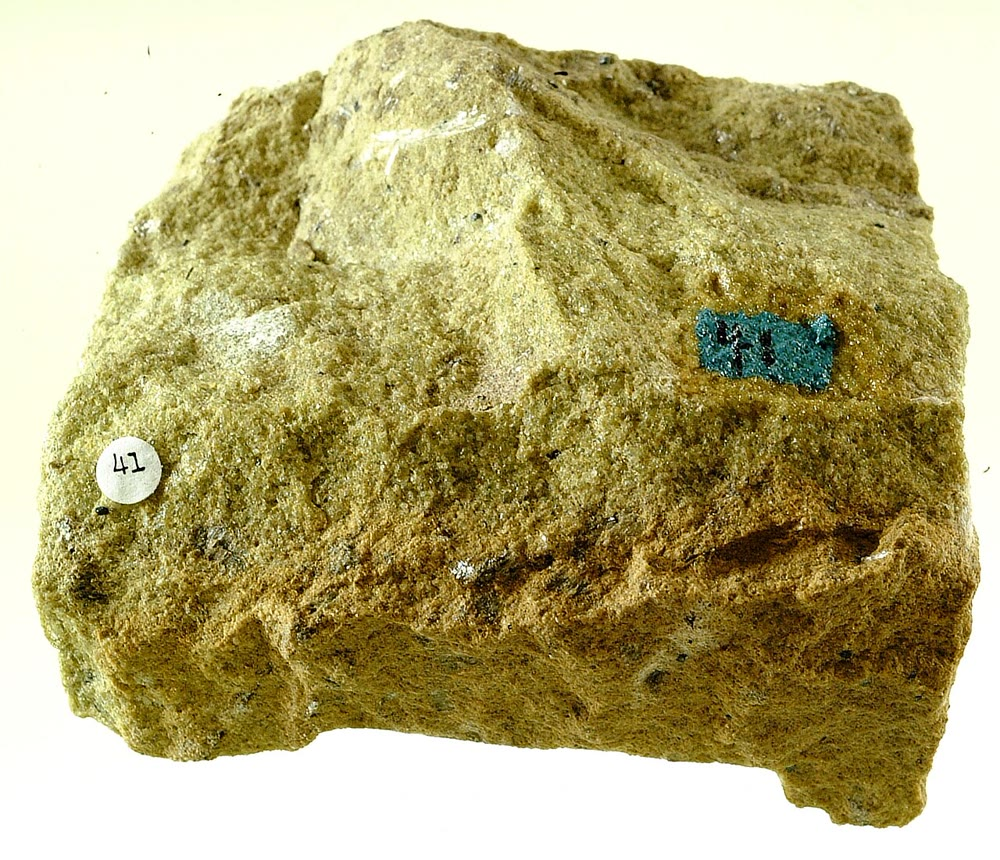
\includegraphics[width=\linewidth]{images/book4/b2-dunite.jpg}
\par\smallskip{\scriptsize एक \omterm{def:b2:mantle-melting:peridotites}{ड्यूनाइट}, लगभग पूरी तरह ओलिवीन, क्रोमाइट के छोटे काले
कणों के साथ; नमूना \qty{8.5}{cm} चौड़ा है (फ़ोटो: Mike Davis, CC0)।}
\end{minipage}
\end{inthefield}
% ledger: casetta23:kimberlite, tulane:ocean-basins (Book 2), bgs:ultramafic

\section{अभ्यास}

\begin{exercise}[$\star$]\label{exo:b2:mantle-melting:1}
ओलिवीन, ऑर्थोपाइरॉक्सीन और क्लाइनोपाइरॉक्सीन के अनुपातों (प्रतिशत) से हर चट्टान का नाम बताइए:
(क) 93, 5, 2; (ख) 75, 25, 0; (ग) 60, 27, 13; (घ) 30, 45, 25। (ङ) मॉडल ऊपरी प्रावार
(57, 28, 13 और \qty{2}{\percent} स्पिनेल) का नाम बताइए, उसके तीन सिलिकेटों को
\qty{100}{\percent} पर पुनः प्रसामान्यीकृत करने के बाद।
\end{exercise}
% ledger: bgs:ultramafic, liang21:dmm-mode

\begin{exercise}[$\star$]\label{exo:b2:mantle-melting:2}
डायोप्साइड--एनॉर्थाइट आरेख पर \qty{60}{\percent} एनॉर्थाइट वाला एक द्रव
ठंडा होता है। (क) वह किस तापमान पर क्रिस्टलित होने लगता है, और कौन-सा खनिज
बनता है? (ख) दूसरा खनिज किस तापमान पर प्रकट होता है, और तब
द्रव का संघटन क्या होता है? (ग) जब
\qty{80}{\percent} डायोप्साइड और \qty{20}{\percent} एनॉर्थाइट वाली चट्टान गरम की जाती है, तो पहले द्रव का संघटन क्या होता है,
और वह किस तापमान पर प्रकट होता है?
\end{exercise}
% ledger: bowen15:di-an

\begin{exercise}[$\star$]\label{exo:b2:mantle-melting:3}
(क) रुद्धोष्म प्रवणता $\alpha T/(\rho c_p)$ केल्विन प्रति गीगापास्कल में परिकलित कीजिए,
$T_p = \qty{1350}{\celsius}$, $\alpha = \qty{4.0e-5}{K^{-1}}$, $\rho =
\qty{3300}{kg/m^3}$, $c_p = \qty{1000}{J/(kg.K)}$ के लिए। (ख) प्रावार के कितने किलोमीटर
एक गीगापास्कल बनाते हैं ($g = \qty{9.81}{m/s^2}$)? प्रवणता को केल्विन
प्रति किलोमीटर में बदलिए और पृष्ठ के निकट की एक सामान्य भूतापीय प्रवणता,
लगभग \qty{30}{K/km}, से तुलना कीजिए।
\end{exercise}
% ledger: katz03:thermo, earle:settings (Book 2)

\begin{exercise}[$\star$]\label{exo:b2:mantle-melting:4}
(क) 0, 1, 2 और \qty{3}{GPa} पर \omterm{def:b2:mantle-melting:peridotites}{पेरिडोटाइट} का शुष्क सॉलिडस परिकलित कीजिए। (ख)
\qty{2}{GPa} के निकट यह प्रति गीगापास्कल कितने डिग्री बढ़ता है? (ग) एक
वाक्य में समझाइए कि \qty{3}{GPa} पर \qty{1400}{\celsius} वाला प्रावार ठोस क्यों है, और
वही प्रावार बिना ऊष्मा-विनिमय के \qty{2}{GPa} तक लाने पर आंशिक रूप से पिघला क्यों है।
\end{exercise}
% ledger: katz03:solidus

\begin{exercise}[$\star\star$]\label{exo:b2:mantle-melting:5}
\qty{70}{\percent} डायोप्साइड और \qty{30}{\percent} एनॉर्थाइट वाला एक द्रव ठंडा होता है।
(क) \qty{20}{\percent} एनॉर्थाइट (\qty{1350}{\celsius}) और \qty{40}{\percent}
(\qty{1277.5}{\celsius}) पर लिक्विडस के बीच अंतर्वेशन करके इसका लिक्विडस तापमान आकलित कीजिए।
(ख) कौन-सा खनिज पहले क्रिस्टलित होता है? (ग) जब द्रव गलनक्रांतिक तक पहुँचता है, तब
तंत्र का कितना द्रव्यमान-अंश क्रिस्टलित हो चुका होता है?
(घ) अंतिम चट्टान में डायोप्साइड और एनॉर्थाइट के अनुपात क्या हैं?
\end{exercise}
% ledger: bowen15:di-an

\begin{exercise}[$\star\star$]\label{exo:b2:mantle-melting:6}
(क) \ce{SiO2} का द्रव्यमान-प्रतिशत परिकलित कीजिए, फ़ॉर्स्टेराइट \ce{Mg2SiO4} में और
एन्स्टेटाइट \ce{MgSiO3} में ($M_{\ce{MgO}} = \qty{40.30}{g/mol}$, $M_{\ce{SiO2}} =
\qty{60.08}{g/mol}$)। (ख) बोवेन और एंडरसन ने पेरिटेक्टिक द्रव को
\qty{97.5}{\percent} \ce{MgSiO3} और \qty{2.5}{\percent} \ce{SiO2} पाया: उसकी
सिलिका-मात्रा क्या है? (ग) उत्तोलक नियम का प्रयोग करके पेरिटेक्टिक पर एन्स्टेटाइट के पिघलने पर
बनने वाले फ़ॉर्स्टेराइट का द्रव्यमान-अंश परिकलित कीजिए, और उनके
\qty{5.5}{\percent} से तुलना कीजिए। (घ) \omterm{def:b2:mantle-melting:peridotites}{पेरिडोटाइट} के गलित की सिलिका-मात्रा के लिए, उसके
ऑर्थोपाइरॉक्सीन की तुलना में, इसका क्या अर्थ है?
\end{exercise}
% ledger: bowen14:mgo-sio2

\begin{exercise}[$\star\star$]\label{exo:b2:mantle-melting:7}
रुद्धोष्म $T = T_p + 20P$ और पाठ के शुष्क सॉलिडस के साथ, वह
दाब और गहराई ($\qty{30.9}{km}$ प्रति गीगापास्कल) परिकलित कीजिए जिस पर गलन शुरू होता है,
(क) $T_p = \qty{1300}{\celsius}$ और (ख) $T_p = \qty{1450}{\celsius}$ के लिए। (ग)
$T_p = \qty{1300}{\celsius}$ के निकट आरंभ प्रति \qty{10}{\celsius} कितने किलोमीटर
गहरा होता है? \cref{prop:b2:mantle-melting:onset} का प्रयोग कीजिए।
\end{exercise}
% ledger: katz03:solidus

\begin{exercise}[$\star\star$]\label{exo:b2:mantle-melting:8}
\qty{2.0}{GPa} पर, \omterm{def:b2:mantle-melting:fraction}{गलन-अंश} को शुष्क सॉलिडस से
\omterm{def:b2:mantle-melting:peridotites}{लर्ज़ोलाइट} लिक्विडस $T_{\mathrm l} = 1475.0 + 80.0P - 3.2P^2$ तक रैखिक रूप से बढ़ता मानिए। $F = 0.10$ के लिए:
(क) पिघलती चट्टान का तापमान परिकलित कीजिए; (ख) $(\partial
T/\partial P)_F$ और $(\partial T/\partial F)_P$ परिकलित कीजिए; (ग) उत्पादकता परिकलित कीजिए,
$c_p = \qty{1000}{J/(kg.K)}$, $\alpha/\rho = \qty{1.21e-8}{m^3/(kg.K)}$ और
$\Delta S = \qty{300}{J/(kg.K)}$ के साथ। (घ) गुप्त ऊष्मा के बिना यह क्या होती?
\end{exercise}
% ledger: katz03:solidus, katz03:melting, katz03:thermo

\begin{exercise}[$\star\star$]\label{exo:b2:mantle-melting:9}
(क) गलित में घुला 1, 5 और \qty{13}{\percent} जल सॉलिडस को कितना
गिराता है? (ख) \qty{1}{GPa} पर जल-संतृप्त सॉलिडस क्या है? (ग) एक प्रावार
द्रव्यमान से \qty{125}{ppm} जल धारण करता है, और खनिजों तथा गलित के बीच जल का
विभाजन गुणांक 0.01 है। बिल्कुल पहले गलन पर गलित $X =
X_{\text{समग्र}}/D$ धारण करता है: इसे और इससे होने वाली सॉलिडस की गिरावट परिकलित कीजिए।
\end{exercise}
% ledger: katz03:water

\begin{exercise}[$\star\star\star$]\label{exo:b2:mantle-melting:10}
(क) \cref{prop:b2:mantle-melting:triangle} में जाँचिए कि हर वर्ष त्रिभुज के आधार में
प्रवेश करने वाला प्रावार उसकी भुजाओं के आर-पार निकलने वाले प्रावार के बराबर है। $U$ पर उठने और $U$ पर निकलने वाले
प्रावार के लिए भुजाएँ \ang{45} पर क्यों होनी चाहिए?
(ख) दिखाइए कि प्रति गीगापास्कल स्थिर उत्पादकता $\Pi$ के साथ, $h_c = \Pi\,\rho
g\,z_0^2/2$ (जहाँ $P_0 = \rho g z_0$), जिससे भूपर्पटी आरंभ की
गहराई के वर्ग के अनुसार बढ़ती है। (ग) एक कटक \qty{50}{mm/yr} की पूर्ण दर से फैलता है और
\qty{7.1}{km} भूपर्पटी बनाता है: कटक का हर किलोमीटर प्रति वर्ष भूपर्पटी का कितना आयतन
बनाता है, और यदि माध्य \omterm{def:b2:mantle-melting:fraction}{गलन-अंश}
\qty{12}{\percent} है तो वह प्रावार का कितना आयतन पिघलाता है?
\end{exercise}

\begin{exercise}[$\star\star\star$]\label{exo:b2:mantle-melting:11}
व्यवस्था-चित्र वाले त्रिघटकी तंत्र में, द्रव $X$ में
\qty{60}{\percent} A, \qty{20}{\percent} B और \qty{20}{\percent} C है;
द्विघटकी गलनक्रांतिक $e_{AB}$ A 40, B 60 (प्रतिशत) पर है, और \omterm{def:b2:mantle-melting:ternary}{त्रिघटकी गलनक्रांतिक} E
A 25, B 30, C 45 पर। (क) द्रव का संघटन लिखिए जब शुद्ध A का द्रव्यमान-अंश $t$
क्रिस्टलित हो चुका हो, और दिखाइए कि B का C से अनुपात 1 पर रहता है। (ख)
$e_{AB}$ से E तक का कोटेक्टिक बिंदुओं $e_{AB} + s(E - e_{AB})$ की रेखा है: ज्ञात कीजिए
कि द्रव उससे कहाँ मिलता है, और तब तक क्रिस्टलित A का अंश। (ग) जब
द्रव E तक पहुँचता है, तो तंत्र का कितना अंश अब भी द्रव है? (C, E से पहले किसी
क्रिस्टल में प्रवेश नहीं करता।) (घ) तब तक कितना A और कितना B क्रिस्टलित हो चुका है?
\end{exercise}

\begin{exercise}[$\star\star\star$]\label{exo:b2:mantle-melting:12}
संतृप्त गलित की जल-मात्रा $X_{\mathrm{sat}} = 12P^{0.6} + P$ है
(प्रतिशत, $P$ गीगापास्कल में)। (क) इसे 1 और \qty{2}{GPa} पर परिकलित कीजिए, इससे होने वाली सॉलिडस की
गिरावट, और दोनों दाबों पर जल-संतृप्त सॉलिडस भी। (ख) 1 और \qty{2}{GPa} के बीच
संतृप्त सॉलिडस लगभग क्यों नहीं बदलता जबकि शुष्क वाला
\qty{100}{\celsius} से अधिक बढ़ता है? (ग) \qty{2}{GPa} और
\qty{1100}{\celsius} पर स्थित प्रावार-कील में, चट्टान के पिघलने के लिए गलित को कितना जल धारण करना होगा?
\end{exercise}
% ledger: katz03:water, katz03:solidus

\section{समस्या: कटक के नीचे}

\begin{problem}[{सप्ताहांत समस्या --- प्रावार रुद्धोष्म से महासागरीय भूपर्पटी की
मोटाई तक, और वापस प्रावार के तापमान तक}]
\label{pb:b2:mantle-melting:1}
प्रावार कटक के नीचे रुद्धोष्म के अनुदिश उठता है और पिघलता है। डेटा: तापीय
प्रसारता $\alpha = \qty{4.0e-5}{K^{-1}}$; घनत्व $\rho = \qty{3300}{kg/m^3}$;
विशिष्ट ऊष्मा $c_p = \qty{1000}{J/(kg.K)}$; गलन की एन्ट्रॉपी $\Delta S =
\qty{300}{J/(kg.K)}$; $g = \qty{9.81}{m/s^2}$; शुष्क सॉलिडस $T_{\mathrm s} =
1085.7 + 132.9P - 5.1P^2$ और \omterm{def:b2:mantle-melting:peridotites}{लर्ज़ोलाइट} लिक्विडस $T_{\mathrm l} = 1475.0 +
80.0P - 3.2P^2$ (\unit{\celsius}, $P$ \unit{GPa} में); फ़िट किए गए गलन-मॉडल की
माध्य उत्पादकता, $\Pi = \qty{9}{\percent}$ प्रति गीगापास्कल; पृष्ठ के निकट क्लाइनोपाइरॉक्सीन
अभिक्रिया गुणांक 0.50; प्रेक्षित भूपर्पटी सामान्य कटकों पर \qty[uncertainty-mode=separate]{7.1 \pm 0.8}{km}
और आइसलैंड प्रावार-स्तंभ के क्रोड के ऊपर \qty{20}{km}। प्रावार
और भूपर्पटी का घनत्व समान मानिए।

\noindent\textbf{भाग I --- गलन कहाँ शुरू होता है।}
\begin{enumerate}
\item $T_p = \qty{1350}{\celsius}$ को केल्विन में बदलिए।
\item रुद्धोष्म प्रवणता $\alpha T_p/(\rho c_p)$ केल्विन प्रति
गीगापास्कल में परिकलित कीजिए, और उसे निकटतम दहाई तक पूर्णांकित कीजिए।
\item प्रावार के कितने किलोमीटर एक गीगापास्कल बनाते हैं? प्रवणता
केल्विन प्रति किलोमीटर में बताइए।
\item रुद्धोष्म $T = 1350 + 20P$ के साथ, आरंभ-दाब
$P_0$ का द्विघात लिखिए और उसे हल कीजिए।
\item वह गहराई और तापमान बताइए जिस पर गलन शुरू होता है।
\item जाँचिए कि $P_0$ पर सॉलिडस वही तापमान देता है।
\end{enumerate}

\noindent\textbf{भाग II --- कितना गलित।}
\begin{enumerate}[resume]
\item \qty{1.5}{GPa} पर सॉलिडस, \omterm{def:b2:mantle-melting:peridotites}{लर्ज़ोलाइट} लिक्विडस और उनका
अंतर परिकलित कीजिए।
\item उनके बीच रैखिक रूप से बढ़ते \omterm{def:b2:mantle-melting:fraction}{गलन-अंश} के साथ, $F = 0.10$ पर चट्टान का
तापमान बताइए, डिग्री सेल्सियस और केल्विन में।
\item वहाँ $(\partial T/\partial P)_F$ और $(\partial T/\partial F)_P$ परिकलित कीजिए।
\item \cref{prop:b2:mantle-melting:productivity} की उत्पादकता परिकलित कीजिए,
प्रतिशत प्रति गीगापास्कल में।
\item फ़िट किया गया मॉडल औसतन $\Pi = \qty{9}{\percent}$ प्रति गीगापास्कल देता है।
यह कम क्यों है? $\Pi$ के साथ, पृष्ठ पर पहुँचा \omterm{def:b2:mantle-melting:fraction}{गलन-अंश} $F_{\max}$
क्या है?
\item मॉडल प्रावार में \qty{13}{\percent} क्लाइनोपाइरॉक्सीन है। पृष्ठ के निकट किस \omterm{def:b2:mantle-melting:fraction}{गलन-अंश}
पर यह खप जाता है? क्या अक्ष के नीचे का अवशेष
\omterm{def:b2:mantle-melting:peridotites}{लर्ज़ोलाइट} है या \omterm{def:b2:mantle-melting:peridotites}{हार्ज़बर्गाइट}?
\end{enumerate}

\noindent\textbf{भाग III --- भूपर्पटी।}
\begin{enumerate}[resume]
\item $H = z_0$ के साथ \cref{prop:b2:mantle-melting:triangle} का प्रयोग करके
भूपर्पटी की मोटाई परिकलित कीजिए।
\item एकत्रित गलित का माध्य \omterm{def:b2:mantle-melting:fraction}{गलन-अंश} क्या है?
\item प्रेक्षित मोटाई से तुलना कीजिए।
\item चित्र का पूरा मॉडल \qty{9.0}{km} देता है। यह आपके आकलन से
पतली क्यों है?
\item दिखाइए कि $h_c = k P_0^2$ और $k$ किलोमीटर प्रति वर्ग
गीगापास्कल में परिकलित कीजिए।
\end{enumerate}

\noindent\textbf{भाग IV --- प्रावार का तापमान।}
\begin{enumerate}[resume]
\item वह आरंभ-दाब $P_0$ परिकलित कीजिए जो \qty{7.1}{km} भूपर्पटी बनाता है।
\item आरंभ की संगत गहराई बताइए।
\item रुद्धोष्म $T = T_p + 20P$ के साथ वह विभव तापमान परिकलित कीजिए जो
आरंभ को उस दाब पर रखता है।
\item 6.3 और \qty{7.9}{km} के लिए गणना दोहराइए: भूपर्पटी का
प्रकीर्णन $T_p$ का कौन-सा परास अनुमत करता है?
\item आइसलैंड प्रावार-स्तंभ के क्रोड के ऊपर भूपर्पटी \qty{20}{km} मोटी है। वहाँ
विभव तापमान परिकलित कीजिए, और प्रश्न~20 वाले पर उसका आधिक्य।
\item महासागरीय द्वीपों के लावा सुझाते हैं कि प्रावार-स्तंभ परिवेशी प्रावार से 200 से \qty{300}{\celsius} अधिक गरम
हैं। सुझाइए कि भूपर्पटी कम आधिक्य क्यों देती है।
\item सामान्य कटक के निकट, \qty{10}{\celsius} अधिक गरम प्रावार के लिए भूपर्पटी कितने प्रतिशत
मोटी होती है?
\item बहुत धीमे कटक पतली भूपर्पटी बनाते हैं। त्रिभुज की सहायता से समझाइए क्यों।
\item भूपर्पटी की मोटाई से मिलने वाला, सामान्य कटक के नीचे के \omterm{def:b2:mantle-melting:tp}{प्रावार का विभव तापमान}
बताइए, जो इस समस्या की मुख्य संख्या है, और उसकी तुलना
खनिज भौतिकी के \qty{1350}{\celsius} और लावा से मिले 1280 से
\qty{1400}{\celsius} के परास से कीजिए।
\end{enumerate}
\end{problem}
% ledger: katz03:solidus, katz03:melting, katz03:thermo, white:crust (Book 3), herzberg:tp (Book 3), katsura:adiabat (Book 3)
